\documentclass[border=10pt]{standalone}
\usepackage{pgfplots}
\pgfplotsset{compat=1.18, trig format plots=rad}
\begin{document}
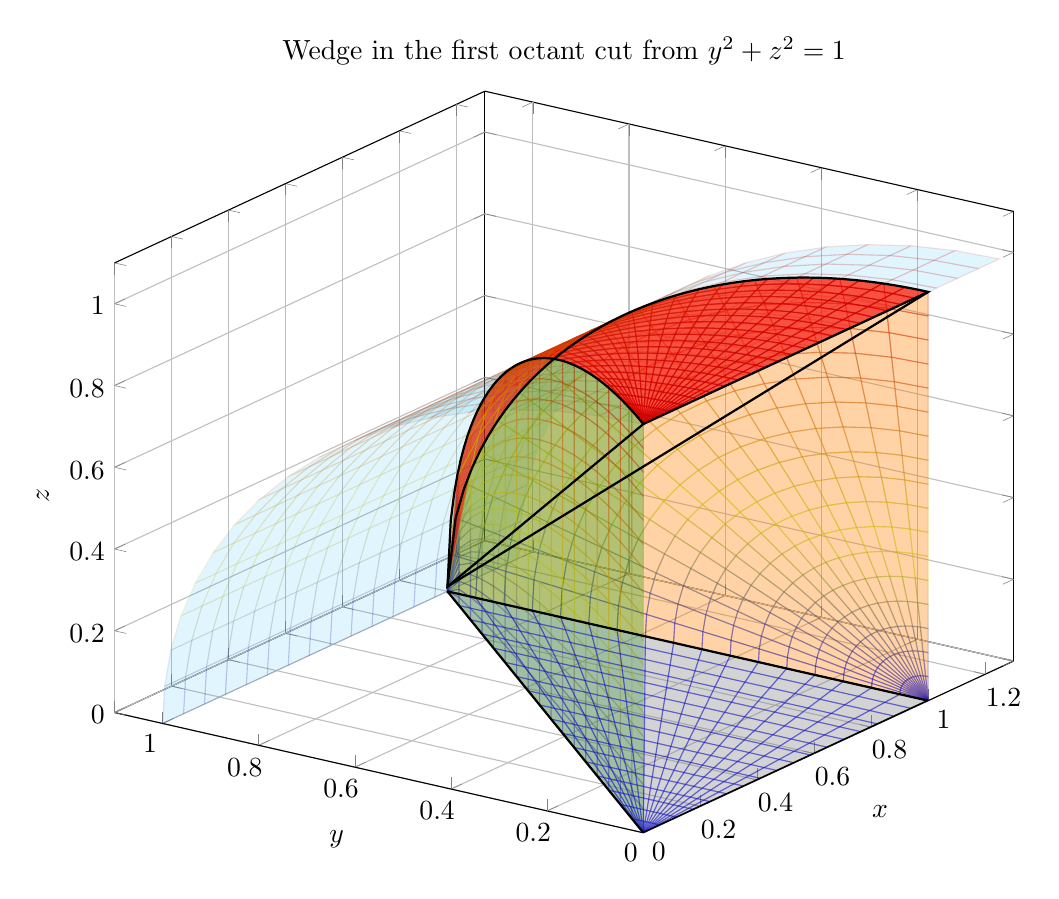
\begin{tikzpicture}
\begin{axis}[
    width=13cm, height=11cm,
    view={-55}{25},
    xlabel={$x$}, ylabel={$y$}, zlabel={$z$},
    xmin=0, xmax=1.3, ymin=0, ymax=1.1, zmin=0, zmax=1.1,
    title={Wedge in the first octant cut from $y^2+z^2=1$},
    grid=major,
]
% Cylinder y^2 + z^2 = 1, first octant, along x-axis
\addplot3[surf, opacity=0.12, draw=none, color=cyan, domain=0:1.25, y domain=0:pi/2, samples=18, samples y=18]
    ({x}, {cos(y)}, {sin(y)});
% Plane x = 1: quarter disk inside the cylinder
\addplot3[surf, opacity=0.35, draw=none, color=orange, domain=0:1, y domain=0:pi/2, samples=18, samples y=18]
    ({1}, {x*cos(y)}, {x*sin(y)});
% Plane y = x
\addplot3[surf, opacity=0.30, draw=none, color=green!60!black, domain=0:1, y domain=0:1, samples=18, samples y=18]
    ({x}, {x}, {y*sqrt(1-x^2)});
% Top surface z = sqrt(1 - y^2) over D: x in [0,1], y in [0,x]
\addplot3[surf, opacity=0.60, draw=none, color=red, domain=0:1, y domain=0:1, samples=22, samples y=22]
    ({x}, {x*y}, {sqrt(1-(x*y)^2)});
% Bottom surface z = 0 over D
\addplot3[surf, opacity=0.35, draw=none, color=gray, domain=0:1, y domain=0:1, samples=18, samples y=18]
    ({x}, {x*y}, {0});
% Key intersection curves
\addplot3[thick, black, domain=0:1, samples=60] ({1}, {x}, {sqrt(1-x^2)});
\addplot3[thick, black, domain=0:1, samples=60] ({x}, {x}, {sqrt(1-x^2)});
\addplot3[thick, black, domain=0:1, samples=10] ({x}, {0}, {0});
\addplot3[thick, black, domain=0:1, samples=10] ({x}, {x}, {0});
\addplot3[thick, black, domain=0:1, samples=10] ({1}, {x}, {0});
\addplot3[thick, black, domain=0:1, samples=10] ({x}, {0}, {1});
\end{axis}
\end{tikzpicture}
\end{document}